\documentclass{school-22.211-notes}
\date{February 22, 2012}

\begin{document}
\maketitle

\topic{Reactor Spectra}
See slides in Lec 4. 

\topic{Resonance Integrals vs. Group Cross Sections}
We introduce \hi{Resonance Integrals} as flux weighted (that is, weight with 1/E spectrum in our case so far because $\phi(E) = \frac{1}{E}$) micro-scopic cross section. RI is used to test accuracy of resonance model. 
\begin{align}
\mathrm{RI} &=  - \int_{u1}^{u2} \sigma(u) \du \\
u &= \ln \left( \frac{E_0}{E} \right) = \ln(E_0) - \ln E \\
\du &= - \frac{1}{E} \dE \\ 
\mathrm{RI} &=  \frac{\int_{E_1}^{E_2} \sigma_{238} (E) \phi(E) \dE}{\int_{E_1}^{E_2} \phi (E) \dE }  \\
\end{align}
Important points:
\begin{itemize}
\item RI is defined directly from cross section data;
\item RI depends on the normalization of the 1/E flux spectrum, but no flux calculation is required because 1/E spectrum is assumed; it is also implicitly assumed that flux equals 1 when $E = 1$ through normalization;
\item For isolated resonances, RI is independent of energy bounds; 
\item Resonance integrals should be independent of temperature. This is because if the energy bound is larger enough, then as temperature increases, the spectrum would broaden, but because the area under the curve remains the same, assume the cross section is constant, then RI is essentially integrating the spectrum, which would not change upon temperature change;
\item RI is useful for inter-comparing libraries or cross section models. It is a classic way to evaluate new resonance data typically from 0.5 eV to 10 keV. We use RI to check our resonance data, in particularly the three big resonances at 6.67, 21, 26 eV. Numerical test of the SLBW RIs shows that the RI comes out to be within 1\% of ENDF/B-VII Reich-Moore data (Lec 6, slide 17, with 0.01 eV as spacing in histogram). 
\end{itemize}

\hi{Group cross section} is a much more useful quantity. From its definition, we see $\sigma_g$ does not depend on the flux normalization: 
\begin{align}
\sigma_g &= \frac{\int_{E_1}^{E_2} \sigma(E) \phi(E) \dE }{\int_{E_1}^{E_2} \phi(E) \dE} 
\end{align}
If we make assumptions on the flux spectrum, then we can relate the group cross section to the effective resonance integral,
\begin{align}
\phi(E) &\sim \frac{1}{E} \\
\sigma_g &= \frac{\int_{E_1}^{E_2} \sigma(E) \frac{1}{E} \dE }{\int_{E_1}^{E_2} \frac{1}{E} \dE} \\
&= \frac{RI'}{\ln(E_2) - \ln(E_1)}  \\
&= \frac{RI'}{\ln(E_2/E_1)} \\
\Aboxed{ RI' &= \sigma_g \ln(E_2/E_1) }
\end{align}
where $RI'$ is not the real RI; it is the effective resonance integral, and it approaches the real RI when $\phi(E)$ approaches $1/E$ (per Reuss' defition, RI refers to infinite U/H ratio, whereas for finite U/H it is effective RI). There are a couple of important points here\footnote{Review here for exam}:
\begin{itemize}
\item Group cross section by definition depends on both cross section and flux spectrum. 
\item Group cross section depends on the flux, but not on the normalization of flux (that is, only the shape matters, not the magnitude);
\item Group cross section depend explicitly on energy bounds (widths) of the groups; 
\item RI can be computed from group cross sections and group energy bounds; As spectrum approaches 1/E, the RI computed from group cross sections will approach true RI. 
\end{itemize}

\topic{Dilution Factor U/H}
As the \hi{Dilution Factor (U/H)} goes to zero, we get infinite dilution, which is what we have been modeling so far. Infinite dilution factor is about 10 or 20 times bigger than a real dilute in a LWR. As the dilution factor increases and approaches a real case, the U238 increases, we would observe more dips in the flux vs. lethargy plot from U238's resonance xs as seen in Figure~\ref{dilution-factor-increase}. 
\begin{figure}
  \centering
  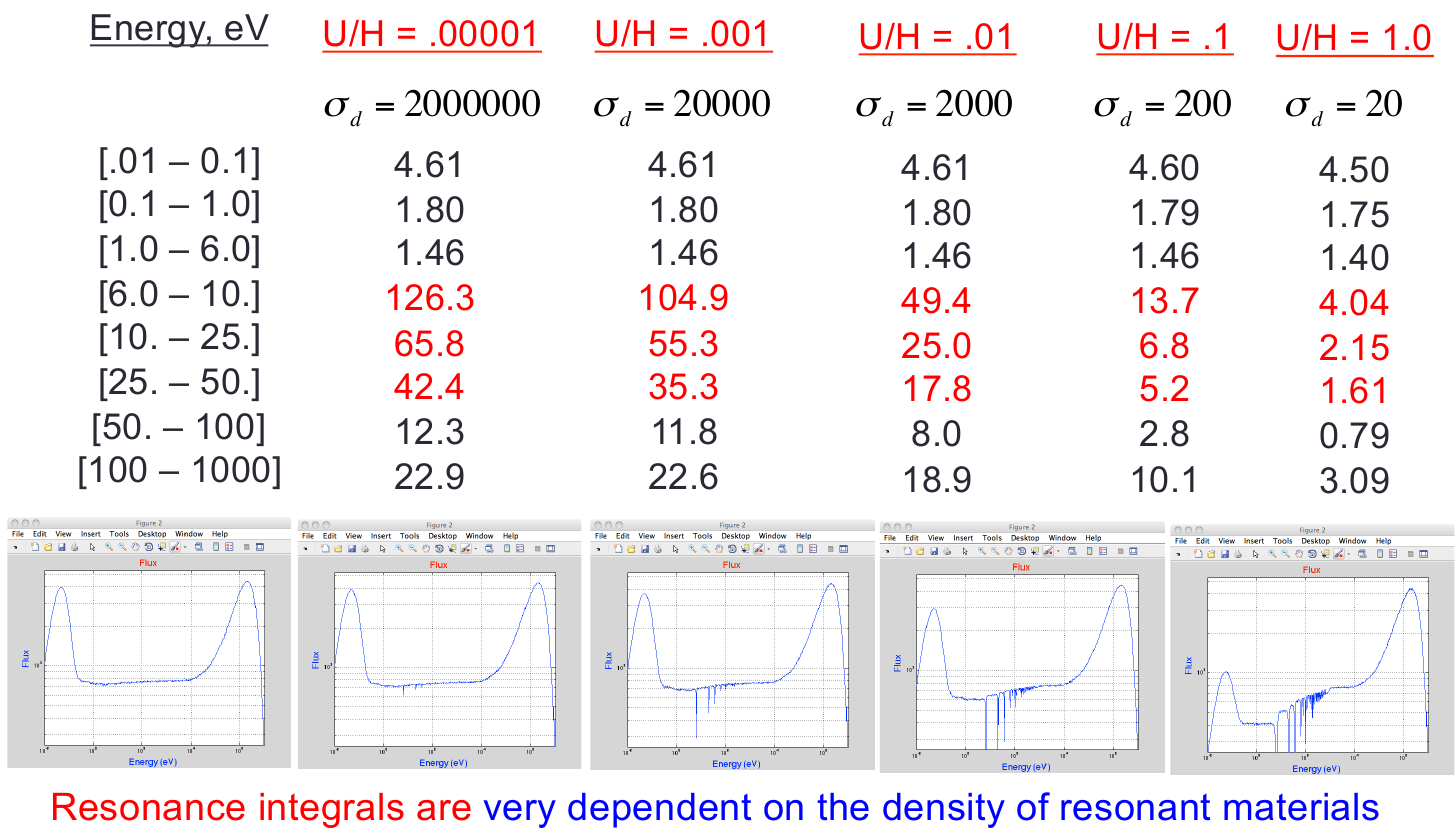
\includegraphics[width=2in]{images/dilution-factor-increase.png}
  \caption{Resonance Dips Increase As U/H Increases} \label{dilution-factor-increase}
\end{figure}
regenerate this graph from slide 15, lec 6. If we zoom in, we still see a 1/E flux spectrum between resonances. insert slide 16, lec 6. 

\topic{Temperature Effects on Cross Section (Doppler Broadening)}
Resonance Integrals increase with increasing temperature. \hi{Doppler Broadening} means, if the width of the spectrum decreases, because the area under the curve stays the same, the depth of the resonance trap would increase and approach infinity eventually, but the probability of neutron slowing down would decrease. 

In general, doppler broadening is the broadening of spectral lines due to the Doppler effect caused by a distribution of velocities of atoms or molecules. There are a couple of different kinds of Doppler broadening, including the thermal Doppler broadening due to the thermal motion of the particles; also, there are broadening depends on the frequency of the spectral line, the mass of the emitting particles, and the temperatures. 

Reference 1: Reuss Section 8.4. 

Reference 2: Handbook of Nuclear Engineering Chapter 4 Section 3. 


Insert Lec 6, Slide 29. 

\textit{At infinite dilution factor, RI is independent of temperature because the area under the psi, chi functions are constant. This is not true at finite concentration of uranium because of self-shielding: as temperature increases, RI would increase.} The fractional change of RI increases as the dilution factor increases. That is, \textit{The higher the concentration, the higher the Doppler Broadening is}. 



\end{document}
